\setcounter{page}{1}
\section*{Zielsetzung}
Der Versuch US $1$ dient als Einführung in die Ultraschalltechnik.
Mit ihm sollen grundlegende physikalische Eigenschaften der
Ultraschallechographie beobachtet und untersucht werden.
\section{Theorie}
\subsection{Schall und Schallausbreitung}
Liegt Schall in einem Frequenzbereich von $\SI{20}{\kilo\hertz}$ bis $\SI{1}{\giga\hertz}$ vor,
wird er als \emph{Ultraschall} bezeichnet. Vom Menschen ist dieser Frequenzbereich nicht wahrnehmbar.
Schall breitet sich als longitudinale Druckwelle $p(x,t)$ der Form
\begin{equation*}
  p(x,t)=p_0+v_0 Z \cos(\omega t - kx) \qquad Z=c\rho
\end{equation*}
aus. Die in der Gleichung auftretende Größe $Z$ bezeichnet die \emph{akustische Impendanz}.
Die Impedanz wird durch die Dichte $\rho$ des durchquerten Materials und der
materialabhängigen Schallgeschwindigkeit festgelegt.
In Flüssigkeiten ist die Schallgeschwindigkeit abhängig von der
Kompressibilität $\kappa$ und der Flüssigkeitsdichte $\rho$
\begin{equation*}
  c\ua{Fl}=\sqrt{\frac{1}{\kappa\rho}}.
\end{equation*}
Statt der Kompressibilität hängt die Schallgeschwindigkeit in einem Festkörper von
dem Elastizitätsmodul $E$ ab:
\begin{equation*}
  c\ua{Fe}=\sqrt{\frac{E}{\rho}}.
\end{equation*}
Zusätzlich wird das Untersuchen von Schall im Festkörper durch Schubspannungen
erschwert. Die Schubspannungen sorgen dafür, dass sich die Schallwelle nicht nur
longitudianl (wie zum Beispiel in Flüssigkeiten), sondern auch als %longitudinal
Transversalwellen ausbreiten.
Außerdem besitzt die Schallgeschwindigkeit in Festkörper eine Richtungsabhängigkeit. %Festkörpern
Ähnlich wie bei elektromagnetischen Wellen können bei Schallwellen auch
Phänomene wie zum Beispiel Reflexion oder Brechung auftreten.

Analog zu anderen Bewegungsvorgängen, treten bei Schallwellen dissipative Effekte auf.
Hierdurch verliert die Welle ein Teil seiner Energie (repräsentiert durch die Intensität $I(x)$) durch die Ausbreitung: %ungünstig formuliert
\begin{equation}
  \label{eq:abfall}
  I(x)=I_0\map{e}^{-\alpha x}.
\end{equation}
Die Größe $\alpha$ ist der Absorptionskoeffizient der Schallamplitude.
Besonders bei Luft ist $\alpha$ groß, deshalb wird bei Anwendung der Ultraschallechographie
ein Kontaktmedium zwischen dem Schallgeber und dem zu untersuchendem Material verwendet.

Beim Auftreffen einer Schallwelle auf eine Grenzfläche wird nur ein Teil der
Welle transmittiert. Der andere Teil wird reflektiert.
Ein Maß für die Reflexion bietet der Reflexionskoeffizient $R$.
Dieser gibt das Intensitätverhältnis zwischen einfallender und reflektierten Welle an.
Er kann mittels der in den anliegenden Materialien vorliegdenden Impendanzen $Z_1$ und $Z_2$
\begin{equation*}
  R=\left(\frac{Z_1-Z_2}{Z_1+Z_2}\right)^2
\end{equation*}
berechnet werden.
Der transmittierte Anteil $T$ lässt sich mit $T=1-R$ ermitteln.

\subsection{Erzeugung und Empfangen von Ultraschall}

Eine Möglichkeit Ultraschallwellen zu erzeugen bietet der \emph{piezo-elektrischen Effekt}.
Befindet sich ein \emph{piezoelektrischer} Kristall (z.\, B. Quarz) in einem elektrischen Feld und steht
zusätzlich eine polare Achse des Krirstalls parallel zum E-Feld, wird dieser %Kristalls
zum Schwingen angeregt. Der schwingenge Kristall strahlt dann Ultraschallwellen ab.
Bei Aneregung des Kristalls mit seiner Resonanzfrequenz ist das erzeugen von Wellen mit hohen %Erzeugen
Schallenergiendichten möglich. %energiedichten
Neben dem Erzeugen bietet der piezoelektrischer Kristall auch die Möglichkeit
als Empfänger von Ultraschallwellen zu fungieren.

\subsection{Methoden der Ultraschallmessung}
Bei Ultraschalluntersuchungen wird das \emph{Durchschallungs-Verfahren} oder
das \emph{Impuls-Echo-Verfahren} verwendet.

Die schematische Darstellung des Durchschallungs-Verfahren ist in Abbildung
\ref{fig: durch} illustriert. Vor und hinter der Probe wird ein Ultraschallsender bzw. -empfänger
platziert.
\begin{figure}[h]
  \centering
  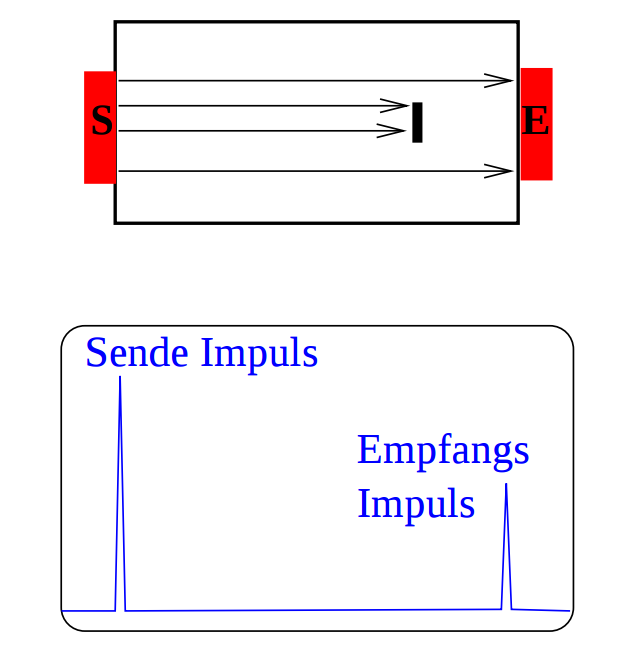
\includegraphics[width=0.4\textwidth]{pics/durchsall.png}
  \caption{Schematische Darstellung des Durchschallungs-Verfahren \cite{anleitungus1}.}
  \label{fig: durch}
  \end{figure}
Der Sender erzeugt kurzzeitige Schallimpulse die vom Empfänger
registriert werden. Befindet sich eine Fehlstelle in der Probe, so misst der Empfänger
eine verringerte Intensität.
Das Verfahren bietet, jedoch keine Möglichkeit die Fehlstelle zu lokalisieren. %kein Komma

Beim Impuls-Echo-Verfahren ist der Sender zeitgleich der Empfänger (vgl. Abb. \ref{fig: echo}).
\begin{figure}[h]
  \centering
  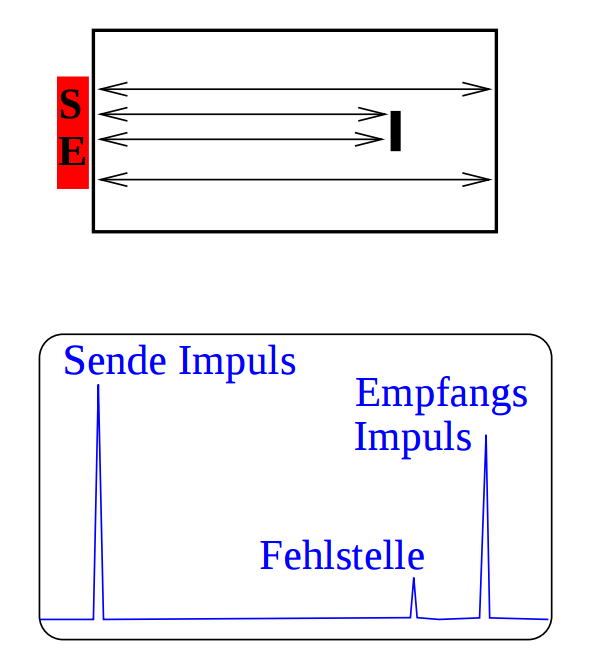
\includegraphics[width=0.4\textwidth]{pics/impuls_echo.png}
  \caption{Schematische Darstellung Impuls-Echo-Verfahren \cite{anleitungus1}.}
  \label{fig: echo}
  \end{figure}
Die erzeugte Schallwelle wird bei der Grenzfläche reflektiert und von der Sonde %an der
empfangen. Mit Hilfe dieses Verfahrens können auch die Orte der Fehlstellen bestimmt
werden. Ist die materialabhängige Schallgeschwindigkeit bekannt, so kann die
Lage der Fehlstelle mit
\begin{equation}
  \label{eq:lage_fehl}
  s=\frac{1}{2}ct
\end{equation}
bestimmt werden.

Um die Ergebnisse einer Ultraschallmessung zu veranschaulichen, werden drei verschiedene
Darstellungsmöglichkeiten verwendet.

Eine Möglichkeit bietet der \emph{A-Scan} (A für Amplitude), in diesem %punkt statt komma
wird die Zeit gegen die empfangene Amplitude aufgetragen.
Ein beispielhafter Verlauf ist in Abbildung \ref{fig: druch} oder \ref{fig: echo}
dargestellt.

Neben dem \emph{A-Scan} gibt es noch den \emph{B-Scan} (B für Brightness).
Bei einem B-Scan wird die Größe der gemessene Amplitude als Helligkeit
auf einem Bild skaliert. Dadurch ist es möglich, ein 2 dim. Bild von der Probe zu erzeugen.

Abschließend bietet der \emph{TM-Scan} (TM bedeutet time motion) die Möglichkeit
Bewegungen in der zu untersuchende Probe darzustellen.
%vielleicht noch erwähnen, dass wir nur a scan gemacht haben
